\documentclass[twoside]{article}
\usepackage[a4paper]{geometry}
\geometry{verbose,tmargin=2.5cm,bmargin=2cm,lmargin=2cm,rmargin=2cm}
\usepackage{fancyhdr}
\pagestyle{fancy}

% nastavení pisma a~češtiny
\usepackage{lmodern}
\usepackage[T1]{fontenc}
\usepackage[utf8]{inputenc}
\usepackage[czech]{babel}

% odkazy
\usepackage{url}

\usepackage{float}
% vícesloupcové tabulky
\usepackage{multirow}
\usepackage{amssymb}
\usepackage{gensymb}
\usepackage{bbold}
\usepackage{mathtools}
\usepackage{commath}

% vnořené popisky obrázků
\usepackage{subcaption}

% automatická konverze EPS 
\usepackage{graphicx} 
\usepackage{epstopdf}
\usepackage{amsmath}
\usepackage{siunitx}
\usepackage{bondgraphs}
\epstopdfsetup{update}

% odkazy a~záložky
\usepackage[unicode=true, bookmarks=true,bookmarksnumbered=true,
bookmarksopen=false, breaklinks=false,pdfborder={0 0 0},
pdfpagemode=UseNone,backref=false,colorlinks=true] {hyperref}

% Poznámky při překladu
\usepackage{xkeyval}	% Inline todonotes
\usepackage[textsize = footnotesize]{todonotes}
\presetkeys{todonotes}{inline}{}
\graphicspath{{./images}}

%https://tex.stackexchange.com/questions/2783/bold-calligraphic-typeface
\DeclareMathAlphabet\mathbfcal{OMS}{cmsy}{b}{n}


% smaz aktualni page layout
\fancyhf{}
% zahlavi
\usepackage{titling}
\fancyhf[HC]{\thetitle}
\fancyhf[HLE,HRO]{\theauthor}
\fancyhf[HRE,HLO]{\today}
 %zapati
\fancyhf[FLE,FRO]{\thepage}

% údaje o autorovi
\title{Modelování a simulace dynamických systémů - semestrální úloha}
\author{Vojtěch Michal}
\date{10. února 2022}

\begin{document}

\maketitle

\section{Úvod}

Repozitář se zadáním modelovací úlohy je dostupný na školním Gitlabu ČVUT \cite{repository}, zadání samotné je dostupné na \cite{zadani}.

\section{Analýza systému}

Laboratorní model přečerpávací vodní elektrárny sestává ze tří nádrží $\text{N}_1$ až $\text{N}_3$ propojených trubkami
s ventily a čerpadlem. Zjednodušené schéma je na obrázku \ref{fig:schema}.

\begin{figure}[htbp]
    \centering
    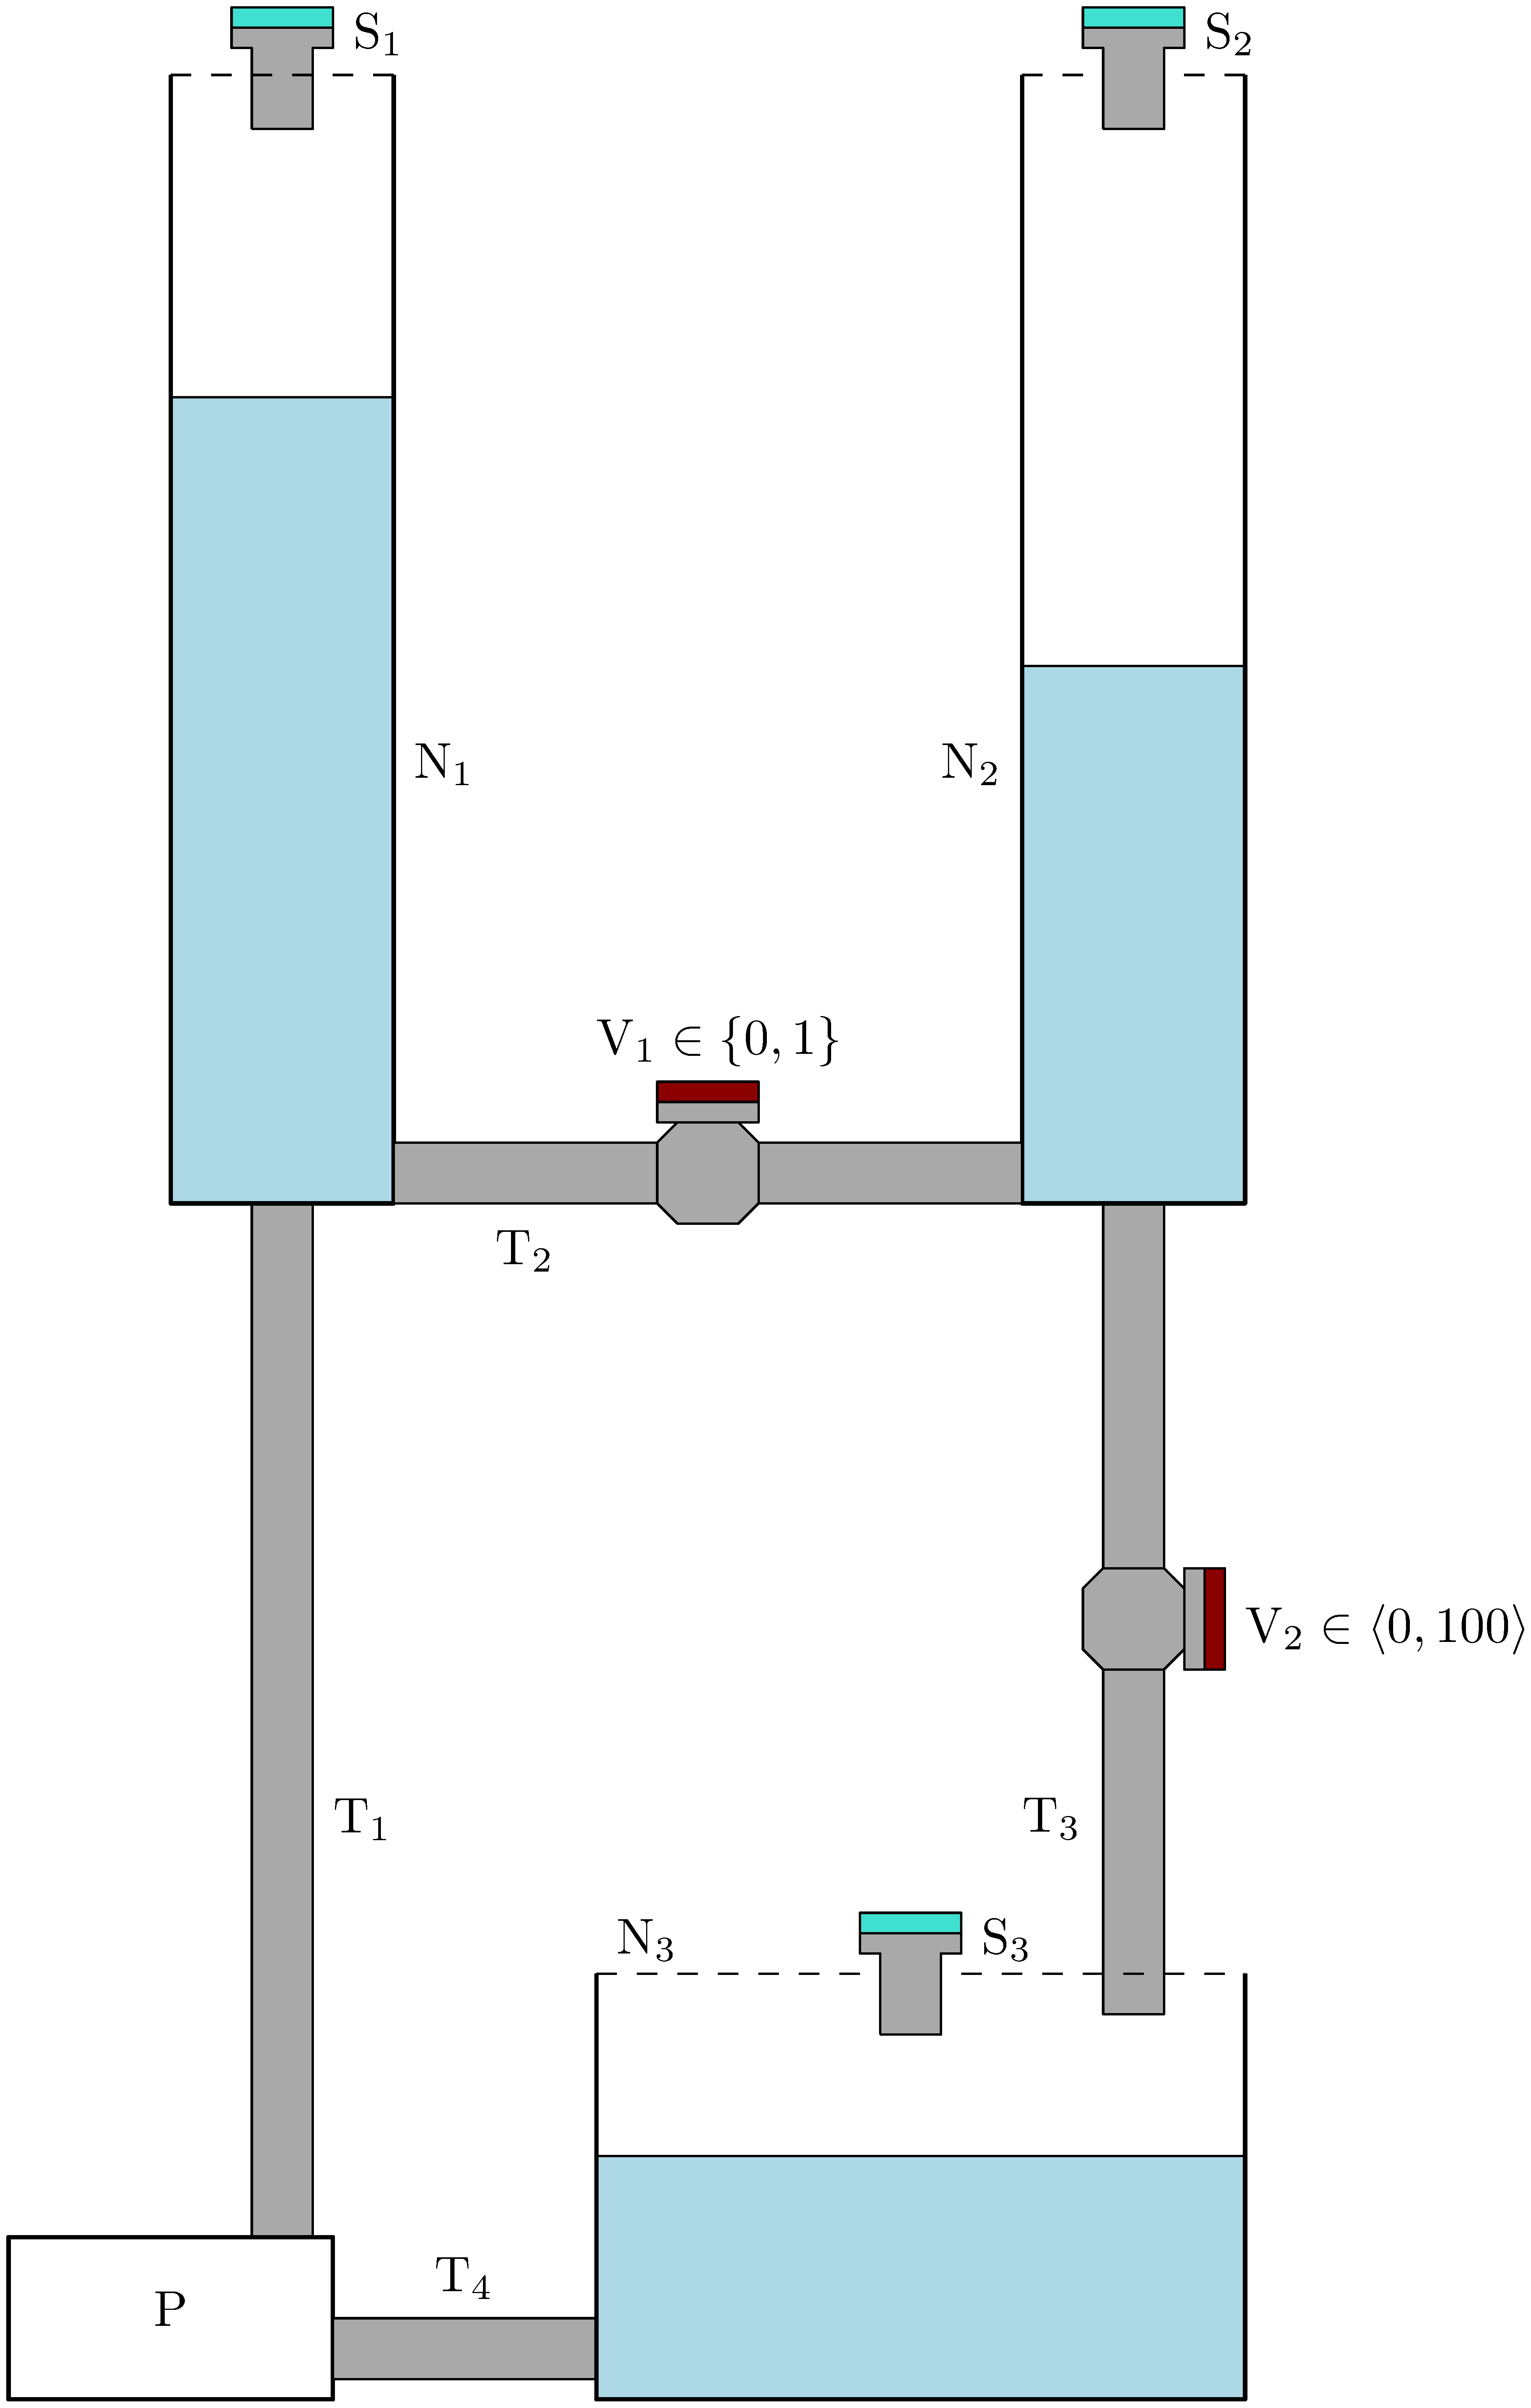
\includegraphics[width=\linewidth]{vodarna_schema.eps}
    \caption{Zjednodušené schéma laboratorního modelu}
    \label{fig:schema}
\end{figure}

\section{Modelování vazebními grafy}

Instancemi \textit{zobecněného úsili} $e$ a \textit{toku} $\dot{q}$ jsou v případě hydrodynamických systémů veličiny tlak $p$ a objemový průtok $Q$.
Pro \textit{zobecněné poddajnosti} je důležitý integrál toku (či též \textit{zobecněné posunutí}) $\int \dot{q} \text{d}t$,
kterým je objem $V$ vody v nádrži. Zobecněné rezistory reprezentují omezení na průtok vody trubkami a ventily.
Místo tlaků uvažuji při řešení problému pouze přetlaky, tedy považuji atmosférický tlak $p_a$ za hladinu nulového úsilí.

\subsection{Nádrže}

Nádrž na vodu v jazyce vazebních grafů modeluje prvek zobecněná poddajnost. Protože nejsou dle zadání shora hermeticky uzavřeny, působí
na vodu atmosferický tlak, vůči kterému je vztažen hydrostatický tlak na dně nádrže. S jeho pomocí lze odvodit modul poddajnosti.

Nechť $V$ označuje objem vody v nádrži o výšce $h$ a ploše podstavy $S$. Nechť $\rho$ je hustota vody
a $g$ je konstanta gravitačního zrychlení. Poté u dna nádrže působí hydrostatický tlak
\begin{equation}
    p = h \rho g = \frac{V}{S} \rho g = V \frac{\rho g}{S}.
\end{equation}
Porovnáním s definičním vztahem pro zobecněnou poddajnost
\begin{equation}
    e = \frac{q}{C}
\end{equation}
je zřejmé, že modul poddajnosti $i$-té nádrže je roven
\begin{equation}
    C_i = \frac{S_i}{\rho g},
    \label{eq:poddajnost}
\end{equation}
kde $S_i$ je plocha dna dané nádrže a $\rho$ i $g$ jsou konstanty uvedné výše.

\subsection{Trubky}

Trubky omezují tok vody po systému, je proto přirozené na ně nahlížet jako na zobecněné rezistory.
Podle \cite{odpor_trubky} platí pro odpor $i$-té trubky vůči toku kapaliny vztah
\begin{equation}
    R_{Ti} = \frac{8\eta L_i}{\pi r_i^4},
    \label{eq:odpor_trubky}
\end{equation}
kde $r_i$ a $L_I$ jsou poloměr a délka dané trubky a $\eta$ je konstanta viskozity,
jež má pro vodu o teplotě 20°C hodnotu $\eta = 1.002 \cdot 10^{-3} \si{\pascal \second}$.

Hodnota odporu $R_{T4}$ mezi spodní nádrží a čerpadlem byla pro malou délku trubky zanedbána.
Trubka $\text{T}_1$ působí v systému odporem tak, jak vychází z rovnice \eqref{eq:odpor_trubky},
naopak odpor trubek $\text{T}_2$ a $\text{T}_3$ je dále ovlivněn ventily na nich umístěnými.
Ventily jsou dále rozebrány v sekci \ref{sec:ventily}.

Trubky $\text{T}_1$ a $\text{T}_3$ jsou umístěny vertikálně a proto v nich je vlivem gravitačního působení Země různý hydrostatický
tlak v různých výškách.
U trubky $\text{T}_3$ je tento fakt zanebán, neboť v ní voda nikdy nestojí. Protože zadání garantuje, že hladina ve spodní nádrži
nikdy nedosáhne po ústí trubky $\text{T}_3$, je trubka (včetně ventilu) modelována jako prostý rezistor limitující průtok a aktivovaná vazba
přenášející objemový průtok přímo do spodní nádrže.

Naopak trubkou $\text{T}_1$ je voda vytlačována vzhůru, jedná se tak o homogenní sloupec vody a u její paty (u čerpadla)
je větší tlak než nahoře u dna nádrže $\text{N}_1$.
Pro modelování tohoto faktu byl na spoj typu 1 reprezentující objemový průtok $Q_1$ připojen zdroj zobecněného úsilí (tlaku)
$\Delta p_{14}$ modelující úbytek vlivem působení hydrostatického tlaku. Tlakový úbytek $\Delta p_{14}$ závisí na výšce sloupce vody
v trubce, bylo by proto vhodné zavést novou zobecněnou poddajnost, jejíž stav by souvisel s výškou vodního sloupce.
Taková struktura modelu by však byla prakticky nepříjemná kvůli interakci poddajnosti trubky a poddajnosti nádrže nad ní umístěné.
Vystižení faktu, že nádrž se může plnit až poté, co je trubka naplněna, by vnášelo do modelu nespojitosti v okamžiku přepínání poddajností.
Vše by bylo dále komplikováno neexistencí senzoru pro výšku sloupce vody v trubce (nepozorovatelný stav) a tedy složitostí verifikace řešení.
Pro implementaci modelu byl použit jednodušší mechanismus a sice řízený zdroj tlaku realizující funkci
\begin{equation}
    \Delta p_{14} = \begin{cases}
        0 & h_1 = 0, \\
        L_1 \rho g & h_1 \neq 0.
    \end{cases}
\end{equation}
Pro použitelnost v numerických simulacích s konečnou přeností výpočtů byla
rovnost s nulou $h_1 = 0$ nahrazena porovnáním $h_1 \le 10^{-4}~\si{\metre}$.

V modelu byla zanedbána setrvačnost vody tekoucí ve všech trubkách. Největší objem má trubka $\text{T}_1$ s hodnotou $2.8419 \cdot 10^{-4} \si{\metre\cubed}$,
při naplnění vodou by se jednalo o 283 gramů vody. S ohledem na fakt, že všechny děje v modelu jsou velmi pomalé (časové konstanty v řádu sekund a více),
byly moduly setrvačnosti zanedbány.


\subsection{Ventily}
\label{sec:ventily}

Ventil $\text{V}_1$ umístěný na trubce $\text{T}_2$ je dvoustavový. Pakliže je otevřený, trubka vykazuje svůj standardní odpor $R_{T2}$.
Pakliže je uzavřený, trubkou nemůže protékat žádná voda a odpor jde limitně do nekonečna. s použitím dvoustavové proměnné $v_1$ definované jako
\begin{equation}
    v_1 = \begin{cases} 
        0 & \text{ventil je uzavřený}, \\
        1 & \text{ventil je otevřený},
     \end{cases}
\end{equation}
lze popsat odpor $R_2$ trubky jednoduchým vztahem
\begin{equation}
    R_2(v_1) = \frac{R_{T2}}{v_1},
\end{equation}
kde dodefinovávám $\frac{x}{0} = \infty$ pro libovolné reálné $x$.

Ventil $\text{V}_2$ umístěný na trubce $\text{T}_3$ lze nastavovat spojitě na 0 až 100 \% otevření a dále vykazuje pásmo necitlivosti
pro hdonoty otevření $\le$ 20~\%.
Nechť $v_2 \in \langle 0, 100 \rangle $ je míra otevření ventilu v procentech. Protože se jedná o proporcionální ventil,
předpokládám popis lineární (nebo lépe řečeno afinní) funkcí. Podmínky
\begin{equation}
    \begin{split}
        R_3(v_2\le20\%) &= \infty, \\
        R_3(v_2=100\%) &= R_{T3},\\        
    \end{split}
\end{equation}
splňuje funkce
\begin{equation}
    R_3(v_2) = R_{T3} \frac{100-20}{\text{max}(v_2, 20) - 20},
\end{equation}
kde opět předpokládám $\frac{x}{0} = \infty$ pro libovolné reálné $x$.

\subsection{Čerpadlo}


\section{Identifikace}

Pro numerické simulace bylo potřeba vyčíslit všechny parametry nalezeného modelu.
K tomu bylo využito dokumentace přiložené mezi podklady k zadání práce.

Na základě tabulek \cite{tabulky} byly určeny hodnoty konstant $\rho = 998~\si{\kilogram\per\metre\cubed}$ a $g=9.81~\si{\metre\per\second\squared}$.

V dokumentaci modelu ve složce \textit{zadani/vodarna/documentace/technicke\_vykresy}
je řada rozměrových schémat zachycujících délky stran nádrží a další hodnoty. Odečtením z rozměrových schémat
byly určeny plochy podstav nádrží 1 až 3 po řadě jako
\begin{equation}
    \begin{split}
        S_1 = S_2 &= (230-15-15)\cdot(330-15-15) \si{\milli\metre\squared}, \\
        S_3 &= (430-15-15)\cdot(1050-15-15) \si{\milli\metre\squared},
    \end{split}
\end{equation}
což po vyčíslení odpovídá modulům poddajnosti
\begin{equation}
    \begin{split}        
        C_1 = C_2 &= 6.1346 \cdot 10^{-6} \si{\metre^4 \second^2\kg^{-1}}, \\
        C_3 &= 4.1715 \cdot 10^{-5}\si{\metre^4 \second^2\kg^{-1}}.
    \end{split}
\end{equation}
Ověřením správnosti postupu budiž fakt, že nádrž $\text{N}_3$ je výrazně větší než nádrže horní,
tedy pojme více toku při stejné změně výšky hladiny, tedy musí mít větší modul poddajnosti.

Na základě rozměrových schémat byly odečteny též rozměry trubek v systému.
S pomocí schématu kompletního modelu byly určeny délky trubek
\begin{equation}
    \begin{split}
        L_1 &= 1900+100-50-229~\si{\milli\metre} = 1.721~\si{\metre},\\
        L_2 &= 680~\si{\milli\metre},\\
        L_3 &= 1900-580-250~\si{\milli\metre}= 1.07~\si{\metre}.
    \end{split}
\end{equation}
Délka trubky $\text{T}_2$ je ve schématu uvedena explicitně. Délky trubek $\text{T}_1$ a $\text{T}_3$ bylo
složitější určit. Dno nádrží $\text{N}_1$ a $\text{N}_2$ se nachází $1.9~\si{\metre}$ nade dnem nádrže $\text{N}_3$,
která je $580~\si{\milli\metre}$ vysoká a má dalších $250~\si{\milli\metre}$ vysoký kryt, což dohromady dává délku trubky $\text{T}_3$.
Délka $\text{T}_1$ je výška dna $\text{N}_1$ nad $\text{N}_3$ plus $100~\si{\milli\metre}$ výšky podložky nádrže mínus výška
podložky pod čerpadlem a mínus výška čerpadla samotného, kterou uvádí datasheet v \textit{vodarna/documentace/cerpadlo} jako $229~\si{\milli\metre}$.

Průměr otvorů pro trubky ve stěnách nádrží má $ 48~\si{\milli\metre}$, nicméně čerpadlo v datasheetu používá rozměr závitu G1,
jehož vnitřní průměr $ 29~\si{\milli\metre}$ byl blíže očekávaným hodnotám odporu trubek.
Pro simulace byl použit průměr trubek pouhých $ \frac{29}{2}~\si{\milli\metre}$ a odpor spočtený podle vzorce \eqref{eq:odpor_trubky}
byl ještě navýšen \todo{finish}




\section{Simulace}

Počáteční podmínky pro jednotlivé simulace byly odvozeny z datasetů přiložených k zadání.
Pro každou simulaci byly odečtením z grafu určeny počíteční výšky hladin v jednotlivých
nádržích, které byly následným vynásobením vektorem ploch podstav převedeny na počáteční podmínky
na objem vody v jednotlivých nádržích.

Výsledný vazební graf popisující systém je vykreslen na obrázku \ref{fig:vazebni_graf}.


\begin{tikzpicture}
    \node[bgelement] (p4) at (0,0) {0};
    \node[bgelement] (p3) at (4,0) {0};
    \node[bgelement] (p1) at (0,4) {0};
    \node[bgelement] (p2) at (4,4) {0};

    \node[bgelement] (Q1_west) at (0,2) {1};
    \node[bgelement] (Q3) at (4,2) {1};
    \node[bgelement] (Q1_south) at (2,0) {1};
    \node[bgelement] (Q2) at (2,4) {1};

    \node[bgelement] (G) at (2,-2) {G:G};
    \node[bgelement] (i) at (2,-4) {1};

    \node[bgelement] (R1) at (2, 2) {R:$R_1$};
    \node[bgelement] (R2) at (2, 6) {R:$R_2(v_1)$};
    \node[bgelement] (R3) at (6, 2) {R:$R_3(v_2)$};
    \node[bgelement] (Rp) at (4,-4) {R:$R_p$};
    \node[bgelement] (I) at (0,-4) {I:$I$};
    \node[bgelement] (setpoint) at (2,-6) {Se:$U_{\text{set}}$};
    \node[bgelement] (delta_p14) at (-2, 2) {Se:$\Delta p_{14}$};
    \node[bgelement] (C1) at (0,6) {C:$C_1$};
    \node[bgelement] (C2) at (4,6) {C:$C_2$};
    \node[bgelement] (C3) at (6, 0) {C:$C_3$};

    \draw[bond,e_out] (p3) -- (Q1_south);
    \draw[bond,e_out] (Q1_south) -- (p4);
    \draw[bond,e_out] (p4) -- (Q1_west);
    \draw[bond,e_out] (Q1_west) -- (p1);
    \draw[bond,e_out] (p1) -- (Q2);
    \draw[bond,e_in] (Q2) -- (p2);
    \draw[bond,e_out] (p2) -- (Q3);
    
    \draw[bond,e_out] (Q2) -- (R2);
    \draw[bond,e_out] (Q3) -- (R3);
    %\draw[effort={0},flow={Q_3},bond,e_out] (Q3) -- (p3); % TODO make activated
    \draw[bond,e_out] (Q1_west) -- (R1);
    \draw[bond,e_in] (Q1_west) -- (delta_p14);

    \draw[bond,e_in] (i) -- (Rp);
    \draw[bond,e_out] (i) -- (I);
    \draw[bond,e_out] (setpoint) -- (i);



    \draw[bond,e_in] (p1) -- (C1);
    \draw[bond,e_in] (p2) -- (C2);
    \draw[bond,e_in] (p3) -- (C3);

    \draw[bond,e_in] (i) -- (G);
    \draw[bond,e_out] (G) -- (Q1_south);

    \label{fig:vazebni_graf}

\end{tikzpicture}
    
\begin{thebibliography}{9}


    \bibitem{repository}
        Repozitář s podklady pro úlohu, \url{https://gitlab.fel.cvut.cz/aa4cc/msd/semestralni-ulohy-pro-predmet-msd/-/blob/master/vodarna}
    \bibitem{zadani}
    Zadání semestrální úlohy, \url{https://gitlab.fel.cvut.cz/aa4cc/msd/semestralni-ulohy-pro-predmet-msd/-/blob/master/vodarna/zadani/msd_vodarna.pdf}
    \bibitem{tabulky}
    Fyzikální tabulky, \url{http://kabinet.fyzika.net/studium/tabulky/tabulky.php}

    \bibitem{odpor_trubky}
    Viscosity and Laminar Flow; Poiseuille's Law, Lumen Physics, \url{https://courses.lumenlearning.com/physics/chapter/12-4-viscosity-and-laminar-flow-poiseuilles-law/}
    
    \end{thebibliography}
    

\end{document}

